% Standalone build of the RunLine QA / Validation Report.
% To submit: copy sections/*.tex and references.bib into the CS 4971 Overleaf
% template and keep its formatting. This preamble only exists so the draft
% compiles locally (tectonic main.tex).
\documentclass[11pt]{article}
\usepackage[margin=1in]{geometry}
\usepackage[T1]{fontenc}
\usepackage{lmodern}
\usepackage{booktabs}
\usepackage{tabularx}
\usepackage{array}
\usepackage{graphicx}
\usepackage{xcolor}
\usepackage{enumitem}
\usepackage[hidelinks]{hyperref}
\usepackage[numbers,sort&compress]{natbib}
\setlist{nosep,leftmargin=1.4em}
\newcolumntype{Y}{>{\raggedright\arraybackslash}X}
\newcommand{\pass}{\textbf{Met}}
\newcommand{\fail}{\textbf{Not met}}
\newcommand{\partmet}{\textbf{Partly met}}
\newcommand{\pending}{\textbf{Pending}}
% Marks a value the team must still fill in or confirm before submission.
\newcommand{\todo}[1]{\textcolor{red}{[TODO: #1]}}

\title{\textbf{RunLine}\\[4pt]\large CS 4971 QA / Validation Report}
\author{RunGuys (Team M3)\\[2pt]
Adithya Balasubramaniam, Krish Patel, Rohan Singh}
\date{\todo{report date}}

\begin{document}
\maketitle

\section{Validation Strategy Overview}

RunLine is a web application that generates running loops. A runner chooses a
start, a target distance, a surface preference (road, mixed or trail) and an
elevation preference (flat, balanced or hilly), and RunLine returns up to three
loops ranked by how well they fit the request. Each route can be downloaded as
GPX for a watch or navigation app. The routing engine searches an
OpenStreetMap walking network \citep{boeing2017osmnx,hagberg2008networkx} with
a cost function that penalizes mapped traffic signals, major-road crossings,
repeated segments, the wrong surface and the wrong amount of climbing.

\paragraph{Definition of success.}
Our Project Proposal \& Plan \citep{runguys2026proposal} defined success as a
runner being able to enter a start and a distance, receive several routes that
stay close to that distance, compare measurable tradeoffs between them, and
export the one they choose. It turned that goal into eleven user stories with
numeric acceptance criteria: seven must-haves (US1 to US7), three
should-haves (US8 to US10) and one nice-to-have (US11). We use those criteria
unchanged as the definition of ``working'' in this report, because they were
fixed before most of the system was built and so cannot have been tuned to
the results. Table~\ref{tab:criteria} restates them. The proposal also set two
technical questions: whether interruption-aware scoring reduces mapped
signals and crossings without losing distance accuracy (US3), and whether the
surface and elevation preferences change the selected routes in the intended
direction (US5, US6).

Two further expectations came from the proposal's discussion of limits rather
than from a user story, and we hold the system to them as well. RunLine must
present route characteristics, never safety guarantees, since OpenStreetMap
can omit crossings, signals and restrictions. It must also avoid retaining
runners' locations, because a start is often a home.

\begin{table}[ht]
\centering\small
\caption{Acceptance criteria from the Project Proposal \& Plan, used as the definition of success.}
\label{tab:criteria}
\begin{tabularx}{\linewidth}{@{}l l Y@{}}
\toprule
ID & Priority & Acceptance criterion (abridged) \\
\midrule
US1 & Must & $\geq$80\% of successful benchmark requests return a top-ranked route within 5\% of the requested distance; all return a route within 10\%. \\
US2 & Must & For $\geq$80\% of requests where the network permits it, at least two candidates overlap by no more than 80\%. \\
US3 & Must & Against a distance-only baseline, median signals plus major-road crossings fall by $\geq$20\% with median distance error $\leq$5\%. \\
US4 & Must & Each candidate shows distance error and the major score components, matching the calculated metrics within display rounding. \\
US5 & Must & Where more than one surface exists, the route moves toward the requested surface relative to the neutral setting in $\geq$75\% of cases. \\
US6 & Must & The hilly route has more elevation gain than the flat route in $\geq$80\% of paired requests. \\
US7 & Must & Ten sampled routes produce GPX that parses without error; one route per distance opens in a GPX-compatible application. \\
US8 & Should & All three team members complete a browser checklist (search, map click, generate, switch, export) without blocking errors. \\
US9 & Should & With a drive radius set, every suggested start lies within the radius and the comparison shows route score and driving cost; ten cases checked. \\
US10 & Should & Warm 3 and 5 mile requests: median below 10\,s, 95th percentile below 20\,s. \\
US11 & Nice & At least one additional area, built with the same pipeline, passes the distance, validity, browser and GPX smoke tests. \\
\bottomrule
\end{tabularx}
\end{table}

\paragraph{Methods.}
We used five validation methods, each chosen for what it can establish about
a route planner and what the others cannot.

\begin{enumerate}
\item \textbf{Automated tests.} A pytest suite and two Node test files check
  the deterministic pieces: distance and overlap calculations, signal and
  crossing counts, repeated-segment detection, scoring, GPX generation, pool
  storage and serving, coverage errors, and the browser's request and
  recording logic. These establish that each component computes what it
  claims to on known inputs. They cannot show that the routes are good.
\item \textbf{A fixed route benchmark measured against the acceptance
  criteria.} Eight public Charlottesville starts at 3, 5, 8 and 12 miles
  (32 requests) are planned under each preference setting, and a script
  computes every numeric criterion (US1, US2, US3, US5, US6, US7 and the local
  part of US10). This is the method the proposal committed to. Because the
  inputs are fixed, it also works as a regression test: our repository rules
  require before-and-after benchmark and shape-audit numbers for any change
  to the routing, scoring or model code before it can be merged.
\item \textbf{An independent audit of the crossing metric.} US3 depends on
  the planner counting major-road crossings correctly, and a metric that only
  agrees with itself proves nothing. We built a separate geometric labeller
  that cuts each route's corridor along major-road centrelines and counts a
  crossing whenever the route moves from one side to the other. We then
  checked it against hand-labelled cases and measured the planner's count
  against its labels.
\item \textbf{Validation of the deployed system.} Scripted requests against
  the public URL check what a runner actually receives: response times
  (US10), coverage in the additional metro areas (US11), closed loops and
  matching GPX, error handling, nearby-start suggestions (US9), and whether
  the numbers the interface displays match the API's metrics (US4).
\item \textbf{Manual review by the team.} The browser checklist (US8), the
  ten nearby-start cases (US9), opening GPX files in an outside application
  (US7) and a three-person route review cover what scripts cannot judge:
  whether the interface is usable and whether a route looks like something a
  runner would actually run.
\end{enumerate}

We deliberately did not run a study with outside participants, as the
proposal stated. Recruiting runners would have required consent procedures
and handling of participants' locations. Our acceptance criteria are also
mostly properties of routes, which a fixed benchmark measures more
repeatably than a small participant group would. The cost is that no
evidence in this report shows that runners other than ourselves find the
routes or the score breakdown useful. We return to this gap in
Sections~\ref{sec:analysis} and~\ref{sec:readiness}.

\paragraph{Scope.}
This report covers \texttt{main} at commit \texttt{f482881}
\citep{runline2026repo} and the production deployment at
\url{https://runline-nine.vercel.app}. When we measured it, the production
backend reported commit \texttt{ebcd150} from 11 November, three code
pull requests behind \texttt{main}. None of them changed scoring, but one
(\#26) changed how loops are generated, so for some requests production can
return different routes from the benchmark, which used \texttt{main}. Charlottesville
is the primary area. Its graph was rebuilt in November to keep signalized
crosswalks, and it is served with a complete set of precomputed routes
(11,417 pools, 605,206 loops). Washington DC, New York, Los Angeles, Atlanta,
Boston and Phoenix are served from a team member's virtual machine and are
covered only as US11 evidence. The stakeholders are the three team members
acting as runners and the course staff. The features covered are loop
generation, preferences, ranking, the comparison interface, GPX export,
nearby starts and start-to-finish routes.

We could not validate several things. In-app GPS run recording was added late
and has only been tested on synthetic location samples, never outdoors on a
phone. We did not audit accessibility (keyboard use, screen readers or
contrast). We did not load-test the deployment with concurrent users. The
metro areas other than Charlottesville were built from an older map graph
that does not keep signalized crosswalks, so their signal counts are less
complete. We also cannot independently verify OpenStreetMap's tags in the
field, so every interruption count in this report means \emph{mapped}
signals and crossings \citep{osmwiki2026signals}.

\section{Validation Artifacts \& Procedures}

Every scripted artifact below lives in the repository \citep{runline2026repo},
takes fixed inputs, and writes its results to a JSON file plus a short
summary. Anyone with the repository and its pinned environment can rerun
them. Appendix~\ref{app:repro} lists the exact commands, and
Appendix~\ref{app:checklists} holds the manual checklists.

\paragraph{Who did the work.}
The team members wrote the requirements, chose the benchmark and its
thresholds, reviewed every change through pull requests, and are responsible
for the manual checks. Much of the measurement tooling (the benchmark
harness, the crossing audit, the pool comparison and the acceptance and
deployment scripts) was written with AI coding assistants (Claude Code and
Codex), which ran under our direction and whose output we reviewed before
merging. \todo{confirm this disclosure matches the course's generative-AI
policy and how each member used these tools.} The automated measurements in
Section~\ref{sec:evidence} were run on \todo{date of final runs} on a MacBook
running Python~3.13 with the exact package versions pinned in
\texttt{requirements.txt}. The pins matter because the saved map graphs only
load under the library versions that built them.

\subsection{Automated tests}
The suite has 223 Python tests across 24 files and 35 Node tests that load the
real browser scripts (\texttt{web/app.js} and \texttt{web/run.js}) into a
sandbox. Table~\ref{tab:tests} groups them by what they protect. Tests build
small synthetic graphs where an answer can be worked out by hand, for example
a straight crossing of a major road versus a turn that stays on the same
side, and they also run complete requests on the shipped Charlottesville
graph. A GitHub Actions workflow runs both suites on every pull request; it
was added during this validation work (pull request \#21), after we found
that only Vercel's preview build had been checking pull requests. A pull
request that broke tests could previously show as passing.

\begin{table}[ht]
\centering\small
\caption{Automated test suite by area (Python unless noted).}
\label{tab:tests}
\begin{tabularx}{\linewidth}{@{}Y r Y@{}}
\toprule
Area & Tests & What it checks \\
\midrule
Graph building and metrics (\texttt{osm}, \texttt{pbf}, signal builders) & 63 & Simplification keeps geometry and signal nodes; crossing, signal and repetition counts on hand-built cases \\
Pool storage and serving & 34 & Format round trips, graph-hash checks, neighbour reads, corrupt or stale pools fall back to live planning \\
Metro tiling and tile serving & 52 & Each cell owned by exactly one tile; tile loading, cache bounds, metro precompute \\
Scoring, planning and coverage & 22 & Penalties applied correctly; preferences change rank; coverage limits reported \\
Start-to-finish routes & 20 & Snapping limits, unreachable or identical endpoints, forwarding rules \\
API, regional forwarding and errors & 16 & Validation errors return explained 4xx; regional outages return 503 \\
GPX and export & 5 & Well-formed GPX whose track matches the route \\
Other (geometry, elevation, starts, privacy, rehearsal) & 11 & Includes a check that the public benchmark file holds no coordinates or addresses \\
Browser logic (Node) & 35 & Request flow, error display, route switching, GPS recording on synthetic samples \\
\bottomrule
\end{tabularx}
\end{table}

\subsection{Route benchmark and acceptance script}
The benchmark uses eight public Charlottesville starts: the Rotunda, the
centre of the map area, and six points 2.5\,km from the centre at 60 degree
intervals. Each start is requested at 3, 5, 8 and 12 miles, giving 32
requests that return up to 96 routes. Private starts that team members use
for their own runs are kept in a git-ignored file and are excluded from every
reported result. The acceptance script (\texttt{scripts/acceptance.py})
plans each request under the default settings (mixed surface, balanced
elevation), then again as road, trail, flat and hilly, and computes each
criterion exactly as Table~\ref{tab:criteria} states it:

\begin{itemize}
\item \textbf{Distance (US1).} Absolute error of the top-ranked route as a
  percentage of the target.
\item \textbf{Alternatives (US2).} For each pair of returned routes, shared
  edge length divided by the shorter route's length; a request passes when
  some pair overlaps by 80\% or less.
\item \textbf{Interruptions (US3).} Mapped signal events plus major-road
  crossings, compared with a \emph{distance-only baseline} planned on the
  same requests. The baseline is a genuine alternative planner, not the
  production one with a setting changed: its path costs are plain edge
  lengths with no signal, crossing or surface penalties, and it ranks only
  by distance error. Both use Dijkstra's algorithm
  \citep{dijkstra1959note}.
\item \textbf{Preferences (US5, US6).} Paired comparisons on the same start
  and distance. A road or trail request ``moves toward'' its surface when its
  trail share is no higher (road) or no lower (trail) than the mixed
  request's. A pair counts for US5 only if the mixed route contains both
  surface types. For US6 the hilly route must have strictly more elevation
  gain than the flat one. Elevation comes from the Copernicus GLO-90 terrain
  model \citep{copernicus2022dem}, baked into the graph when it is built.
\item \textbf{GPX (US7).} Ten routes are sampled across the four distances.
  Each file is parsed and validated against the official GPX~1.1 schema
  \citep{topografix2004gpx}, and its track must be closed and match the
  route's reported length within 1\%.
\item \textbf{Speed, local (US10).} Wall time per request after the map is
  loaded, for 3 and 5 miles.
\end{itemize}

The script runs twice: once against the live planner alone, and once through
the deployed serving path, which answers from precomputed routes first and
plans live only when none fit. The second run measures what a runner actually
receives. The graph's hash is recorded with the results so they can be tied
to the exact map they came from.

\subsection{Shape and crossing audits}
\texttt{scripts/shape\_audit.py} plans 96 routes from a ring of starts and
records properties that the acceptance criteria do not mention but that make
a route bad to run: roundness, measured as $4\pi A/L^2$ (the Polsby--Popper
score \citep{polsby1991third}, where 1 is a circle and below 0.2 is close to
an out-and-back), whether the route enters a dead end, short revisits, and the
share of its length that repeats.

\texttt{scripts/audit\_crossings.py} provides independent labels for US3. For
each stretch of route that touches a major road, it draws a 15\,m corridor
with at least 50\,m of travel on either side, cuts it along the road's
centreline, and counts a crossing when the route passes from one piece to the
other. Grade-separated passes are excluded. The planner's own count is then
scored against these labels for precision and recall. The labeller never calls
the planner's crossing rule, so the two can disagree, and when they did we
plotted each disagreement and settled it by inspecting the map.

\subsection{Precomputed route (pool) check}
\texttt{scripts/compare\_pools.py} draws 40 starts at random (seed 7) within
6\,km of the Charlottesville centre and requests 3, 5, 6.5, 8 and 12 miles on
all three surfaces: 600 requests. It records whether the precomputed routes
could answer, how long that took, and the same quality metrics as the
benchmark, so answers from pools can be compared with live planning on the
same requests.

\subsection{Deployed-system validation}
\texttt{scripts/validate\_deployed.py} sends requests to the public URL one at
a time with a pause between them, using public landmark starts only, and
caps the total at about 250 requests to stay polite to the shared servers.
For US10 it times 3 and 5 mile requests at ten Charlottesville starts, twice
each, reporting the first request at each start separately as a cold start.
For US11 it requests 3, 5 and 8 miles from public landmarks in each metro
area and checks that each loop is closed, in the distance band, and has a GPX
file whose track matches the route. For US9 it runs ten nearby-start cases
across 1, 3 and 5 mile radii and checks every suggested start against the
radius. For US4 a Node harness feeds real responses captured from production
into the interface's own rendering code and compares every number shown on a
route card with the API's metrics. Separately,
\texttt{scripts/presentation\_check.py} replays ten fixed scenarios, including
error cases and address autocomplete, and confirms each GPX file matches its
drawn route.

\subsection{Manual checks}
Three procedures need a person. Each team member runs the browser checklist
in Appendix~\ref{app:checklists} (US8) in a desktop browser and on a phone,
recording pass, fail or notes for each step. The team opens at least one GPX
file per distance in an outside application and records whether the track
appears correctly (US7). Each member also independently reviews the same
twelve benchmark routes against a five-point checklist covering continuity,
backtracking, unreasonable crossings, map rendering, and agreement between
the drawn route and its metrics. Disagreements are discussed and the outcome
recorded.

\subsection{Consent, privacy and accessibility}
No outside participants took part, so no consent was needed. Privacy shaped
the procedures in three ways. Only public landmarks appear in tracked files
and in this report, and a test fails the suite if coordinates or addresses
appear in the public benchmark file. The application keeps no account,
history or saved requests. A recorded run stays in the page's memory and is
discarded when the page closes \citep{w3c2026geolocation}. Map data is
OpenStreetMap's, used under the Open Database License with attribution
\citep{osm2026copyright}. We did not evaluate accessibility, which is listed
as a gap in Section~\ref{sec:analysis}.

\section{Evidence \& Findings}
\label{sec:evidence}

Table~\ref{tab:matrix} summarizes the result for every acceptance criterion.
The rest of this section gives the evidence behind each row, then the
findings from the audits that the criteria do not cover. Unless stated
otherwise, benchmark figures come from the acceptance run of
\todo{date, e.g. 17 November 2026} on code \texttt{61f45cd} (main
\texttt{f482881} plus the measurement script, no routing changes) and the
rebuilt Charlottesville graph (hash prefix \texttt{66b524897627167e}), which
is the graph production serves. The script reports two modes. \emph{Live} is
the planner on its own, with precomputed routes switched off. \emph{Served}
is the path the API actually uses: precomputed routes first, live planning
if none fit. In the served run, precomputed routes answered 30 of the 32
default requests.

\begin{table}[ht]
\centering\small
\caption{Acceptance criteria results. ``Live'' is the planner alone; ``served'' is what the API returns.}
\label{tab:matrix}
\begin{tabularx}{\linewidth}{@{}l Y Y l@{}}
\toprule
ID & Live planner & Served / deployed & Status \\
\midrule
US1 & 29/32 (90.6\%) within 5\%; 32/32 within 10\% & 32/32 within 5\% & \pass \\
US2 & 32/32 with a distinct pair & 31/32 (96.9\%) & \pass \\
US3 & Median interruptions 14 $\rightarrow$ 4 ($-$71\%); error 1.45\% & 14 $\rightarrow$ 3 ($-$79\%); error 0.95\% & \pass \\
US4 & \multicolumn{2}{l}{Values match API (0 of 3,969 differ); all 8 components shown (fixed 18 Nov)} & \pass \\
US5 & 62/64 (96.9\%) toward preference & 63/64 (98.4\%) & \pass \\
US6 & 21/32 (65.6\%), 11 ties & 26/32 (81.2\%), 6 ties & \partmet \\
US7 & 10/10 valid against GPX 1.1 schema & 10/10; outside-app import \todo{team} & \partmet \\
US8 & \multicolumn{2}{l}{Team checklist \todo{results}; automated browser tests 35/35} & \pending \\
US9 & \multicolumn{2}{l}{19/19 starts in radius; score and drive cost shown (fixed 18 Nov)} & \pass \\
US10 & Laptop: median 0.33\,s, p95 1.18\,s & Production: median 0.48\,s, p95 1.95\,s & \pass \\
US11 & \multicolumn{2}{l}{6/6 areas: 72/72 requests, 216 valid routes} & \pass \\
\bottomrule
\end{tabularx}
\end{table}

\subsection{Route generation (US1, US2)}
All 32 default requests returned routes in both modes. In live mode, 29 of
32 top-ranked routes (90.6\%) were within 5\% of the target and all 32 were
within 10\% (median error 1.45\%, worst 7.87\%), which meets US1. The three
misses were all 3 mile requests (6.0\%, 7.9\% and 6.6\%). They are not
ranking mistakes. The planner treats any route within $\pm$0.25 miles as on
target and then ranks mainly on interruptions, and 0.25 miles is 8.3\% of
3 miles. The proposal's 5\% threshold is stricter than the product's own band
at short distances, and we discuss this mismatch in
Section~\ref{sec:analysis}. In served mode all 32 top routes were within 5\%
(worst 4.59\%).

For US2 we measured overlap as shared edge length divided by the shorter
route's length. Every live request returned at least one pair of routes
overlapping by 80\% or less (median lowest overlap 0.10). In served mode
31 of 32 did. The exception returned only two routes, which shared 81.4\% of
the shorter one. The planner kept both because its own duplicate test
divides shared length by the \emph{combined} length (0.67, under its 0.70
limit). The two measures disagree when routes differ in length, so a pair
the planner considers distinct can fail the proposal's definition.

\subsection{Fewer interruptions (US3)}
The distance-only baseline was planned on the same 32 requests, with plain
edge lengths as path costs and ranking by distance error alone.
Table~\ref{tab:us3} compares it with RunLine. Interruptions are mapped signal
events plus major-road crossings, counted two ways: by the planner itself
and by the independent geometric labeller. Both counts fell by more than
70\%, far past the 20\% bar, while median distance error stayed at 1.45\%
(the baseline's was 0.61\%). Across all top routes, the total went from 507
interruptions to 108 by the planner's count, and from 458 to 105 by the
geometric labels. RunLine had fewer interruptions than the baseline on 28 of
32 requests, the same on 3, and more on 1 (a 3 mile request from the
north-east ring start).

\begin{table}[ht]
\centering\small
\caption{US3: median signals plus major-road crossings of the top-ranked route, 32 requests.}
\label{tab:us3}
\begin{tabular}{@{}l r r r r@{}}
\toprule
Distance & Baseline & RunLine & Baseline error & RunLine error \\
\midrule
3 mi & 4.5 & 1.0 & 0.38\% & 2.98\% \\
5 mi & 10.5 & 2.5 & 0.74\% & 1.50\% \\
8 mi & 17.0 & 4.0 & 0.29\% & 1.38\% \\
12 mi & 32.0 & 5.5 & 0.82\% & 0.93\% \\
\midrule
All (live) & 14.0 & 4.0 ($-$71\%) & 0.61\% & 1.45\% \\
All (geometric labels) & 13.0 & 3.0 ($-$77\%) & & \\
\bottomrule
\end{tabular}
\end{table}

The trade is visible in the error column. Avoiding interruptions costs
distance accuracy, most at 3 miles, where there are fewest alternative
streets. It stays well inside the 5\% limit.

The crossing count deserves its own scrutiny, since US3 is only as good as
it. On the rebuilt graph, the planner's crossing count agreed with the
geometric labels with precision 0.974 and recall 1.000 over 264 matched
events: seven crossings counted that the labels did not support, and none
missed. Building the labeller changed the product. Its first version cut a
single corridor for the whole route, and wherever a route passed under a
bridge elsewhere, that corridor joined the road's two sides and hid real
crossings. Plotting the disagreements showed that eight of nineteen apparent
planner errors were labeller errors, including a residential street straight
across a major road. The labeller now cuts each stretch on its own corridor.
The same review found a real gap in the planner: walking along a major road
past a major side road was not counted, although a pedestrian has to cross
that side road. We added that rule and a test for it.

\subsection{Preferences (US5, US6)}
In every default request the top route used both surfaces, so all 32 starts
and distances counted for US5. Trail requests raised the median trail share
from 0.50 to 0.85, and road requests lowered it to 0.14. Across the 64
paired comparisons, 62 (96.9\%) moved toward the requested surface live and
63 (98.4\%) served, which meets the 75\% bar.

US6 is the one must-have that is not fully met. The hilly route climbed more
than the flat route in 21 of 32 live pairs (65.6\%), short of 80\%. Served, it
did in 26 of 32 (81.2\%), which passes by a single pair. In no pair did the
hilly route climb \emph{less} than the flat one. Every miss is a tie, where
both settings returned the same top route. The cause is in the design. The
elevation preference changes only the final ranking, not the path search, so
flat and hilly requests choose from the same candidates. It also carries the
smallest ranking weight (1.5, against 6 for signals and 5 for repetition), so
once interruptions and shape are accounted for it rarely decides the order.
In one 3 mile case the hilly ranking still put a 231\,ft route first, ahead
of alternatives climbing 372 and 414\,ft that also had no interruptions. The
median top-route gain was 581\,ft flat and 646\,ft hilly: the preference
works in the intended direction, but weakly.

\subsection{Export (US7)}
Ten routes sampled across the four distances all parsed and validated against
the official GPX~1.1 schema (checked with \texttt{xmllint}), and every track
was closed and matched its route's length. We then checked every route in the
run, 576 live and 474 served, with the same result. The length check is
nearly circular, since the reported distance is computed from the same points
the file contains. It shows that no points were lost or duplicated, not that
the distance itself is right. \todo{Outside-application import: name the app,
the four routes tried and the outcome.}

\subsection{Speed (US10, local part)}
On a laptop with the map already loaded, warm 3 and 5 mile requests took a
median of 0.33\,s (95th percentile 1.18\,s) from the live planner and 0.07\,s
(0.36\,s) when served from precomputed routes. Loading the map took 0.16\,s
and the first live request 1.19\,s. These numbers isolate the software and
exclude the network and the hosting platform, which the deployed measurements
below include.

\subsection{Deployed system (US4, US8, US9, US10, US11)}
We sent about 230 requests to the public site on the evening of 16 November
(Eastern time), one at a
time. None returned a server error, and all eight deliberately invalid
requests (missing start, zero or excessive distance, unsupported area and
similar) returned an explained 4xx message. The deployed page and script were
byte-identical to \texttt{main}. After the interface fix described below we
reran the display and nearby-start checks on 18 November (68 requests); the
deployed page again matched \texttt{main}.

\paragraph{Displayed values and score components (US4).}
US4 has two halves, and on 16 November the deployed interface met only the
first. We fed 126 real production responses through the interface's own
rendering code and compared every number shown on the 378 resulting route
cards with the API's metrics: 4,284 checks with no mismatches. The second half
failed. Cards showed distance, mapped signals, climb and trail share. The
scorer combines eight components (distance, signals, major-road crossings,
surface, elevation, repetition, shape and driving). The interface showed only
signals as a count, showed distance, surface and elevation indirectly, and did
not show major-road crossings, repetition, shape, driving, the distance error,
or any score. The repository history explains how this happened. A line
reading ``signals $\cdot$ major crossings $\cdot$ \% repeated'' was added on
11 November and removed the same day in a change that simplified the
interface, and the score breakdown the proposal described was never built.
Our automated tests checked that displayed values were correct but not that
the required ones were present, so neither change failed a test.

We fixed this on 18 November (\#29). Each card now shows major-road crossings
and a line with the distance off target, the repeated share and the score.
The selected route's panel adds an expandable ``Why this rank'' list of all
eight components, each with what it measured and its points, which sum to the
score (Figure~\ref{fig:app}). The change also added browser tests that fail
if any of these fields disappears. We then reran the same deployed check (68
requests, 18 November): 50 production responses rendered into 150 cards gave
3,969 displayed values with no mismatches, and all eight components were
shown with their points. US4 is now met.

\begin{figure}[ht]
\centering
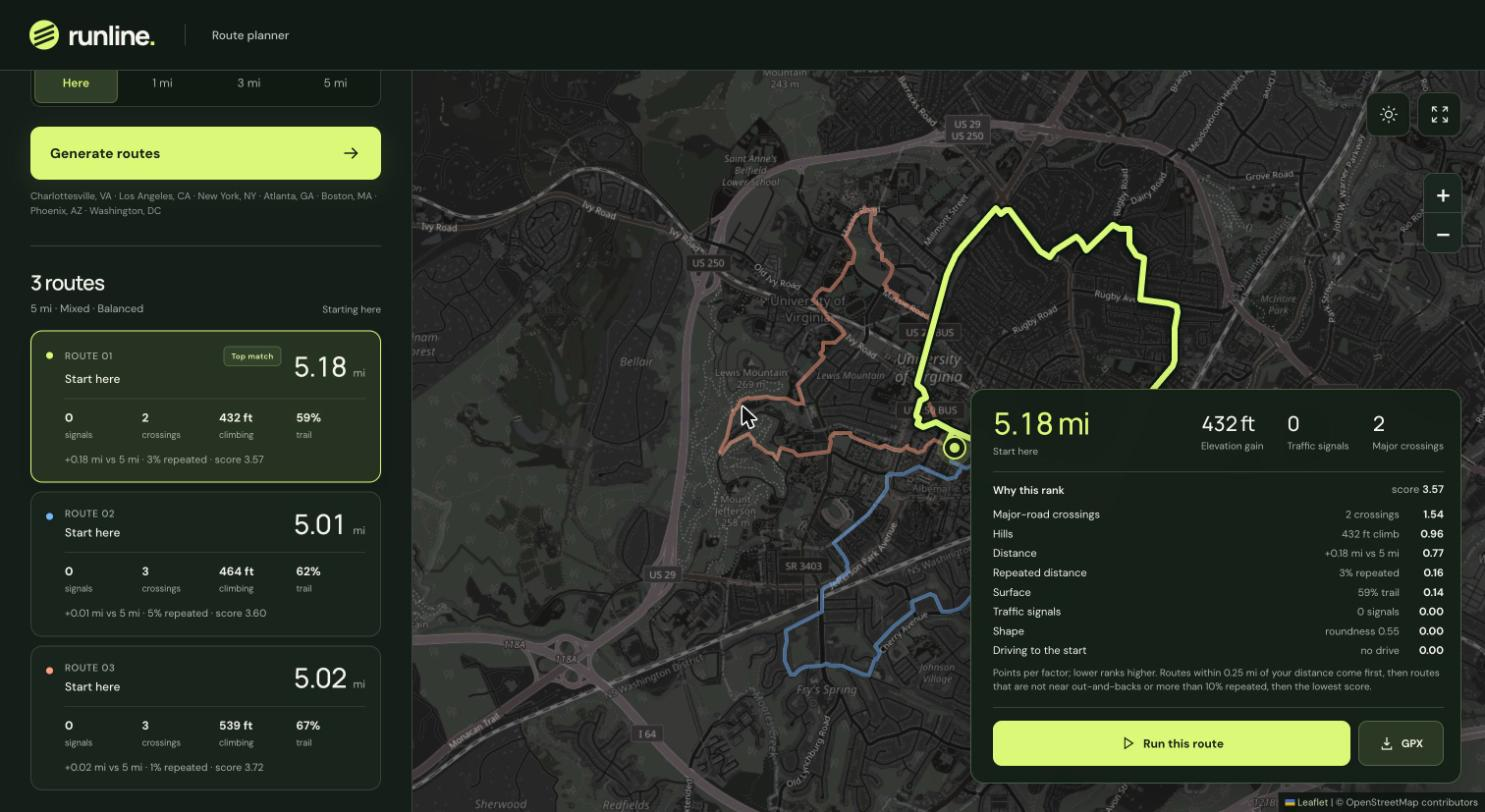
\includegraphics[width=\linewidth]{figures/app-results.jpg}
\caption{The deployed interface after a 5 mile request from the Rotunda
(18 November, after the fix). Each card shows crossings, distance off target,
repetition and score; the panel's ``Why this rank'' list gives every scoring
component's measurement and points.}
\label{fig:app}
\end{figure}

\paragraph{Nearby starts (US9).}
Ten Charlottesville cases across 1, 3 and 5 mile radii returned 19 routes
from alternative starts, and none lay outside the selected radius by road or
straight-line distance. On 16 November the interface named the alternative
start and said how many nearby starts were checked, but showed neither the
route's score nor the added driving distance, so the comparison US9 asks for
was not visible. Since the 18 November fix each alternative-start card shows
its driving distance and score, and the panel says how far to drive to the
start. The rerun repeated all ten cases with the same result (19 routes, none
outside the radius) and confirmed both values are displayed.
These requests always plan live and took a median of 15.2\,s (worst
24.0\,s). In 5 of the 19 routes the reported driving distance was
\emph{shorter} than the straight-line distance, because it is measured
between the nearest road-network points and leaves out the short legs onto
the network. A fix (\#33) adds those legs: over all 37,061 pairs of a public
park and a shipped start within 3 miles of it, the drive was below the
straight line in 380 pairs before and in none after.

\paragraph{Response time (US10).}
Table~\ref{tab:latency} gives end-to-end times measured from a laptop
through the public site. Warm 3 and 5 mile requests met the criterion easily
in every area: a median of 0.48\,s and a 95th percentile of 1.95\,s over 66
requests. The slowest warm request took 14.0\,s (Los Angeles). First requests
in an area were slower, because the server has to load that part of the map,
and two first requests (Boston and New York, both typed addresses that also
had to be geocoded) took over 20\,s. US10 covers warm requests only, so these
do not fail it, but a runner opening the app in a new city meets exactly this
case.

\begin{table}[ht]
\centering\small
\caption{US10: production response times, 3 and 5 mile loops (seconds, end to end).}
\label{tab:latency}
\begin{tabular}{@{}l r r r r l@{}}
\toprule
Area & Warm $n$ & Median & p95 & First request (median / worst) & Pool / live \\
\midrule
Charlottesville & 30 & 0.46 & 0.77 & 0.45 / 3.9 & 29 / 1 \\
Washington, DC & 6 & 0.45 & 6.09 & 6.8 / 7.0 & 6 / 0 \\
New York & 6 & 0.89 & 2.02 & 18.3 / 20.3 & 2 / 4 \\
Los Angeles & 6 & 0.61 & 14.04 & 6.9 / 7.0 & 6 / 0 \\
Atlanta & 6 & 0.33 & 0.74 & 4.5 / 5.0 & 6 / 0 \\
Boston & 6 & 0.51 & 0.60 & 5.6 / 23.1 & 6 / 0 \\
Phoenix & 6 & 0.36 & 0.59 & 7.0 / 7.1 & 6 / 0 \\
\midrule
All areas & 66 & 0.48 & 1.95 & & \\
\bottomrule
\end{tabular}
\end{table}

\paragraph{Additional areas (US11).}
All six metro areas passed every smoke check: 72 requests at 3, 5 and 8 miles
from public landmarks returned 216 routes, every one closed, within the
$\pm$0.25 mile band, and with a GPX file matching its geometry point for
point. Between 34 and 36 of each area's 36 routes were within 5\% of the
target, and all were within 10\%. For all 378 loop routes collected across
the run, the score we recomputed from each route's metrics matched the API's
order. The browser half of US11 is covered by the team checklist.

\paragraph{Supporting evidence for US8.}
Scripts confirmed that place search returned suggestions for five public
names, that picking one moved the start, and that a typed address and a map
click at the same point produced identical routes. A start-to-finish request
in Charlottesville returned a correct 3.48 mile path in 1.7\,s. These checks
support US8 but do not replace the three-person checklist the proposal
specifies, whose results are \todo{fill in from Appendix~\ref{app:checklists}}.

\paragraph{A defect found by the validation tooling.}
Both of our own rehearsal scripts failed against the public site before
making a single route request, while passing against the backend directly.
The cause is the place-list endpoint: the hosting platform's cache returns
it Brotli-compressed even to clients that only accept gzip, which browsers
handle but ordinary HTTP libraries do not. Runners are unaffected, but any
non-browser client, including our monitoring, is. On 18 November the same
cache returned gzip to every client, including one that asked for no
compression. The public site's \texttt{/api} route forwards to the backend,
and the platform's cache for that forwarding stored the backend's
already-compressed answer for whichever client asked first; the backend's own
cache was correct. Turning off caching on the forwarding route (\#34) gave
each client its requested encoding on a preview deployment.

\paragraph{A weak live answer.}
One 3 mile request from a park start was answered live with three routes
that were all close to out-and-backs (roundness 0.13), two of them repeating
23\% of their length. Live planning uses the 10\% repetition limit only to
order routes, not to exclude them. On 16 November the interface did not show
repetition at all; since the 18 November fix each card shows the repeated
share. To see how often this happens we planned live from all 48 public park
starts at 3 and 5 miles: 12 of the 95 answers showed at least one such route,
and in none of them was a rounder route within twice the distance tolerance
left unshown, because ranking already puts every rounder in-band route first.
Excluding these routes would therefore only return fewer of them, so the fix
(\#32) adds a notice instead: ``No rounder loop of this length was found
from this start'', with the count when only some routes are affected.

\subsection{Findings outside the acceptance criteria}
\paragraph{Route shape.}
The criteria do not mention route shape, but a route can pass all of them and
still be unpleasant to run. Of the 96 live routes in the default run, 93 were
within the $\pm$0.25 mile band, 8 had a roundness below 0.2 (close to an
out-and-back), and 12 repeated more than 10\% of their length. The median
route repeated 2.2\%. Served routes were cleaner: all 95 were in band, 2 had
roundness below 0.2 and 4 repeated more than 10\%, because precomputed routes
that repeat too much are filtered out when they are generated. The separate
shape audit on the rebuilt graph found no route entering a dead end, but
three with a short revisit, up from none on the previous graph.

\paragraph{Precomputed route coverage.}
On the 600-request check against the deployed Charlottesville data,
precomputed routes answered 548 (91.3\%): 184 mixed, 181 road and 183 trail.
The other 52 were planned live, which took a median of about 1.4\,s on the
requests we timed, against 64\,ms from precomputed routes. All 52
came from 7 of the 40 starts. Two of those starts missed on every request. One
had its nearest map point on a four-node fragment disconnected from the
street network. The other had no good loop at all, and live planning did
poorly there too (38\% repeated distance). A fix that retries from the nearest
connected point and searches a wider ring of cells raised the rate to
582/600 (97.0\%) with identical results for the earlier hits. It is written
and tested (pull request \#15) but not yet deployed.

\paragraph{Privacy.}
Reviewing the code for what it stores, we found no database, account or
request history. We did find two log lines that record location. When
pre-loading a map fails, the API logs the runner's exact start coordinates,
and when a precomputed route is unusable it logs the 200\,m cell the request
fell in. Neither is stored by RunLine, but the hosting platforms keep logs.
Both lines now name the area instead (\#31), with tests that fail if a log
line contains a start's coordinates or cell.

\paragraph{Map data.}
Rebuilding the Charlottesville graph to keep signalized crosswalks raised the
number of signal nodes from 131 to 569, and counted signal events on the
benchmark rose from 38 to 74. This is not a regression in routing. The old
graph had dropped the crosswalk signals during simplification, so earlier
signal counts were undercounts. The six other metro areas still use graphs
built before this fix.

\section{Analysis \& Action Plan}
\label{sec:analysis}

\paragraph{Against the definition of success.}
The routing engine meets the goal the proposal set for it. Requests return
loops close to the requested distance (US1), with real alternatives (US2), and
with a quarter to a third of the interruptions a distance-only planner would pick
(US3), at a distance cost well inside the limit. The surface preference works
reliably (US5), GPX output is valid (US7), the system is fast once warm
(US10), and the same pipeline now serves six more metro areas (US11). The
first validation run found the result weaker at the point where the runner
meets the engine. The proposal promised that a runner could ``compare
measurable tradeoffs'' and ``make the final choice'' themselves (US4), and on
16 November the interface did not show most of the tradeoffs the engine was
making. We fixed that display on 18 November and the rerun passed. Of the
seven must-haves, six are now met and US6 is met only through the served
path. One should-have is incomplete: US8 waits on the team checklist.

\paragraph{Priorities.}
We ranked issues by how much they affect what a runner sees and by whether
they break a must-have criterion. The two display gaps ranked first, so we
fixed them first. They were the only failures a runner would notice on every
request, and they undid the project's stated difference from existing tools,
which is that the tradeoffs are visible. The weak elevation preference ranks
next. It is a must-have, and
a runner who asks for hills and gets the same route as ``flat'' will conclude
the setting does nothing. Deployment issues follow, because several fixes are
already written but not live. Map-data and scaling issues rank lower. They are
real, but they mostly affect the metros beyond our primary area.

\paragraph{Decisions.}
Table~\ref{tab:actions} records a decision for each important finding. Owners
follow the areas of responsibility in our proposal: the interface for
Adithya, data, performance and deployment for Krish, and routing and scoring
for Rohan. Each item names how we will check that it worked. In every case
the check reruns the same script that found the problem, so a fix is not
counted until the measurement that failed passes.
\todo{Team to confirm owners and target dates.}

\begin{table}[ht]
\centering\footnotesize
\caption{Decisions on the main findings.}
\label{tab:actions}
\begin{tabularx}{\linewidth}{@{}>{\raggedright\arraybackslash}p{2.6cm} >{\raggedright\arraybackslash}p{1.5cm} Y l >{\raggedright\arraybackslash}p{3.1cm}@{}}
\toprule
Finding & Decision & Action & Owner & How we will verify \\
\midrule
US4: crossings, repetition, distance error and score not shown & Completed fix (\#29) & Restored crossings; added distance off target, repetition and score to each card and an expandable score breakdown & Rohan & Deployed rerun 18 Nov: 3,969 values, 0 mismatches, 8/8 components shown \\
US9: drive cost and score not shown & Completed fix (\#29) & Show driving distance and score on alternative-start cards and in the panel & Rohan & Ten-case rerun 18 Nov: both shown, 19/19 in radius \\
US6: hilly often ties flat & Design change & Let elevation influence path search, not only ranking, then retune its weight & Rohan & \texttt{acceptance.py}: US6 $\geq$80\% live \emph{and} US3 still met \\
Production backend behind \texttt{main}; manual deploys & Planned fix & Merge the reproducible release script (\#18) and redeploy from a recorded commit & Rohan & \texttt{/api/version} equals the release commit \\
Precomputed routes miss 8.7\% of requests & Completed fix, not deployed & Retry from the connected network and a wider ring (\#15) & Rohan & 600-request check $\geq$97\% after deploy \\
Live answers can be all slivers or repeat 23\% & Planned fix & Exclude routes over the repetition limit when alternatives exist; otherwise show a notice & Rohan & Shape audit; the failing park case \\
Place list served Brotli to non-browser clients & Planned fix & Stop the cache serving one encoding to every client & Krish & Both rehearsal scripts pass against the public site \\
Start locations written to logs & Planned fix & Log the area name instead of coordinates or cells & Rohan & Test that fails if a log line contains coordinates \\
Tests did not catch removed UI fields; no CI on PRs & Completed fix & Tests run on every pull request (\#21); browser tests now assert the US4 and US9 fields are present (\#29) & Rohan & CI blocks a PR that removes a required field \\
First request in a new city up to 23\,s & Backlog & Compact tile format (\#22) and pre-loading the map when a start is chosen & Krish & Deployed first-request times \\
Metros use graphs without crosswalk signals & Deferred & Rebuild with the signal-preserving builder in the next cluster batch & Krish & Signal-node counts and benchmark per metro \\
US1 5\% rule vs.\ the $\pm$0.25 mile band & Explicit decision & Keep the band; the 3 mile misses are deliberate trades for fewer interruptions & Rohan & Report both measures \\
US2 overlap definition differs from the code & Backlog & Align the duplicate test with the shorter-route measure & Rohan & US2 served rerun \\
Drive distance can be below straight line & Backlog & Add the legs from each start onto the road network & Rohan & US9 check: road $\geq$ straight line \\
\bottomrule
\end{tabularx}
\end{table}

\paragraph{Limits of the evidence.}
Several limits qualify every conclusion above.
\begin{itemize}
\item \textbf{One city.} The benchmark is 32 requests from eight starts in a
  single city. It was fixed before the system was tuned, but it is small, and
  the metro checks used six warm requests per area, where the 95th percentile
  is just the slowest request.
\item \textbf{Mapped interruptions only.} Signals and crossings are counted
  from OpenStreetMap \citep{osmwiki2026signals}. The crossing audit shows the
  planner counts what the map contains, not that the map is complete. Fewer
  signals is also not the same as safer, since a signal may protect a
  crossing.
\item \textbf{Self-built ground truth.} The crossing labels came from our own
  geometric labeller. We checked it against hand-labelled cases and inspected
  every disagreement, but it is not an independent survey.
\item \textbf{Elevation resolution.} Elevation comes from a 90\,m terrain
  model \citep{copernicus2022dem}, which captures hills but not short, steep
  grades.
\item \textbf{Test conditions.} Production timings come from one network
  path at one time of day, with no concurrent users.
\item \textbf{No outside users.} No runner outside the team has used
  RunLine under observation. Whether the tradeoffs, once displayed, actually
  help someone choose is untested, and so is whether our ranking matches
  what runners prefer.
\end{itemize}

\section{Reflection on Readiness}
\label{sec:readiness}

\paragraph{What is reliable now.}
For a runner in Charlottesville who looks at a route before running it,
RunLine is ready to use. The evidence for that is strong and repeatable. Every
benchmark request in both modes returned routes, distance fit met its
criterion, interruptions fell by more than 70\% against a distance-only
planner, the surface preference moved routes the right way in 97 to 98\% of
cases, every GPX file we generated validated, and warm requests answer in
under a second. The precomputed routes served in production are on average
better than live planning: all were within the distance band and fewer
repeated themselves. The six additional metro areas passed the same smoke
checks, which shows the pipeline generalizes beyond the city it was tuned on.

\paragraph{What remains uncertain.}
Until 18 November the engine was ahead of the interface: a runner saw a good
route but not why it was chosen, which is the part of the design the proposal
said distinguished RunLine. That display is now in place and verified, but no
runner outside the team has used it yet. The elevation preference works in the right direction
but too weakly to rely on. The production backend is several changes behind
the code we measured, and two finished fixes (higher precomputed coverage and
the reproducible release) are not live. We also have no evidence about
people other than ourselves, and none about the GPS run mode outdoors or about
accessibility.

\paragraph{What must happen before wider use.}
In order: redeploy the
backend from a recorded commit with the precomputed-coverage fix; complete the
three-person browser checklist, the GPX import check and the route review;
remove start locations from logs; and run an accessibility review against a
recognized checklist. Before anyone outside the team is invited to use it, we
would also want a short observed session with a handful of runners. The
proposal's premise was that visible tradeoffs help a runner choose, and
nothing in this report tests it. The metro
areas should not be promoted beyond a preview until they are rebuilt with the
crosswalk signals and the first request in a new city is reliably fast.

\paragraph{What validation taught us.}
Three lessons changed how we work. The first is that a metric needs a check
that does not share its assumptions. Building the independent crossing
labeller found errors in both directions: the labeller was wrong in eight of
the cases we first blamed on the planner, and the planner was missing a whole
class of crossings. Without the audit, the US3 result would rest on a count
nobody had checked. The second is that tests prove what they assert and
nothing else. Our interface tests confirmed that every displayed number was
correct, and so stayed green when the numbers that mattered most for US4 were
removed from the screen. Measuring against the proposal's criteria, rather
than against our tests, is what exposed it, and it is why our browser tests now
check that required fields are present and why tests run on every pull request. The third
is that the deployed system is its own thing to validate. The backend was
behind the code we benchmarked, and a caching behaviour broke our own
rehearsal scripts while leaving browsers unaffected. Neither shows up on a
laptop. The validation plan for the final sprint therefore reruns the
acceptance and deployment scripts against production after every release,
not only the test suite before it.


\bibliographystyle{plainnat}
\bibliography{references}

\appendix
\section{Reproducing the measurements}
\label{app:repro}

All commands run from a checkout of the repository \citep{runline2026repo}
with its pinned environment
(\texttt{pip install -r requirements.txt -e '.[dev,build]'}). Results are
written to the git-ignored \texttt{output/} directory.

\begin{small}
\begin{verbatim}
python -m pytest -q -rs                                # Python suite (223 tests)
node --test tests/web_flow.mjs tests/run_session.mjs   # browser logic (35 tests)
python scripts/acceptance.py --data <dir with graphs/ and pools/>
                                    # US1-US3, US5-US7, US10 (local); seed 4971
python scripts/shape_audit.py                          # roundness, dead ends, repeats
python scripts/audit_crossings.py                      # independent crossing labels
python scripts/compare_pools.py                        # 600-request pool check, seed 7
python scripts/validate_deployed.py --pause 1.0 --budget 250
                                    # US4, US9, US10, US11 against production
node scripts/ui_display_check.mjs output/deployed-validation   # US4/US9 UI checks
python scripts/presentation_check.py --api <url> --require-pool
\end{verbatim}
\end{small}

\noindent The acceptance results were produced on code \texttt{61f45cd}
with the rebuilt Charlottesville graph (SHA-256 prefix
\texttt{66b524897627167e}) and its matching complete pool file. The
deployed-system run was on 16 November against backend commit
\texttt{ebcd150}. Full tables, definitions and per-case outputs are in
\texttt{docs/acceptance.md} and \texttt{docs/deployed-validation.md} in the
repository.

\section{Manual checklists}
\label{app:checklists}

\subsection{US8 browser checklist}
Each member runs this once on a desktop browser and once on a phone, at
\url{https://runline-nine.vercel.app}, using only public starts. Record P
(pass), F (fail, with a note) or N/A.

\begin{table}[ht]
\centering\small
\begin{tabularx}{\linewidth}{@{}r Y c c c@{}}
\toprule
\# & Step & Adithya & Krish & Rohan \\
\midrule
1 & Search for ``Rotunda'' and pick the suggestion; the pin moves there. & & & \\
2 & Click elsewhere on the map; the start moves to the click. & & & \\
3 & Request 5 miles, mixed, balanced; routes appear without an error. & & & \\
4 & Switch between the route cards; the map highlights the chosen route. & & & \\
5 & Change surface to trail and regenerate; the results change or a notice explains why not. & & & \\
6 & Change elevation to hilly and regenerate; the climb shown changes or a notice explains why not. & & & \\
7 & Download GPX for the selected route; a file is saved. & & & \\
8 & Enter an invalid distance (0 or blank); an explained error appears. & & & \\
9 & Choose a start outside the supported areas; an explained error appears. & & & \\
10 & Use Start $\rightarrow$ finish with two points in Charlottesville; a one-way route appears. & & & \\
\bottomrule
\end{tabularx}
\end{table}

\subsection{US7 GPX import}
For one route at each of 3, 5, 8 and 12 miles, import the downloaded file into
an outside application \todo{name the application, e.g. Garmin Connect,
Strava or gpx.studio} and record whether the track appears, whether its
distance matches RunLine's within 2\%, and whether start and finish meet.

\subsection{Route review}
Each member independently marks twelve benchmark routes (three starts
$\times$ four distances, routes listed in the acceptance output) on five
questions: (1) the route is continuous; (2) it has no obvious backtracking;
(3) it has no crossing a runner would refuse; (4) it renders correctly on the
map; (5) the displayed metrics agree with what the map shows. Disagreements
are discussed and the agreed outcome recorded.

\section{Detailed results}
\label{app:results}

\paragraph{US11 per area.} Routes within 5\% of target out of 36 (12 requests
at 3, 5 and 8 miles, three routes each). All 216 were closed, within the
$\pm$0.25 mile band and within 10\%, with matching GPX.

\begin{center}\small
\begin{tabular}{@{}l r l@{}}
\toprule
Area & Within 5\% & Answered from \\
\midrule
Washington, DC & 36/36 & precomputed \\
New York & 35/36 & 4 of 12 precomputed, 8 live \\
Los Angeles & 36/36 & precomputed \\
Atlanta & 34/36 & precomputed \\
Boston & 35/36 & precomputed \\
Phoenix & 34/36 & precomputed \\
\bottomrule
\end{tabular}
\end{center}

\paragraph{US6 ties (live).} The eleven pairs where flat and hilly returned
the same top route: ring\_060 5\,mi; ring\_120 3 and 12\,mi; ring\_180 3, 5, 8
and 12\,mi; ring\_240 5, 8 and 12\,mi; ring\_300 3\,mi. No pair had the hilly
route climbing less. After the 18 November fix (\#38) no pair tied; in three
the flat route climbed more (ring\_120 3\,mi, 355 vs 231\,ft; ring\_240 8\,mi,
868 vs 728\,ft) or the same (ring\_300 3\,mi, 231\,ft).

\paragraph{Manual checklists.} \todo{Attach the completed US8 checklists, GPX
import record and route review from Appendix~\ref{app:checklists}.}


\end{document}
